\documentclass[12pt]{article}                  % base article class
\usepackage[osf,sups]{Baskervaldx}             % baskerville, lining figures
\usepackage[bigdelims,baskervaldx]{newtxmath}  % baskerville math
\usepackage{graphicx}
\usepackage[hidelinks=false]{hyperref}


\setlength{\parindent}{0pt}         % no paragraph indentation
\setlength{\parskip}{7pt}           % spacing between paragraphs


\def\parens#1{\left(#1\right)}

\begin{document}

\begin{center}
	\Huge The Kernel Rank Transform

	\large Rafael Grompone von Gioi, Enric Meinhardt-Llopis
\end{center}

\bigskip

\section{Introduction}

%Recall the original definition of the rank transform in a discrete setting
%(put reference).
The rank and census transforms were introduced in 1994 by
Zabih-Woodfill~\cite{ZW} as pre-processing steps to improve the performance
of patch-matching for stereo vision algorithms.
Using the same notation as the original authors, the rank transform of a
digital image~$P\mapsto I(P)$ is defined as the
digital image
\begin{equation}\label{eq:rt}
	R(P) = \left\|\left\{
		P'\in N(P)\ |\ I(P')< I(P)
	\right\}\right\|
\end{equation}
where~$N(P)$ is a square neighborhood of size~$d\times d$ around the pixel~$P$.
In other words,~$R(P)$ is the number of pixels in the neighborhood
whose intensity is less than the intensity of the central pixel.
Notice that, by construction,~$R(P)$ takes integer values in the
set~$\{0,\ldots,d^2-1\}$.
%The original motivation for the rank transform was a pre-processing of
%images before patch-matching for stereo vision (?).

%SCRIPT ./krt square3 f/x.png  |qeasy 0 1 - f/x_sq3.png
%SCRIPT ./krt square10 f/x.png |qeasy 0 1 - f/x_sq10.png
%SCRIPT ./krt square40 f/x.png |qeasy 0 1 - f/x_sq40.png
\begin{figure}[p]
	\begin{tabular}{ll}
		\includegraphics[width=0.49\linewidth]{f/x.png} &
		\includegraphics[width=0.49\linewidth]{f/x_sq3.png} \\
		Image $256\times256$&
		$N=3$ \\
		&\\
		\includegraphics[width=0.49\linewidth]{f/x_sq10.png} &
		\includegraphics[width=0.49\linewidth]{f/x_sq40.png} \\
		$N=10$ &
		$N=40$ \\
	\end{tabular}
	\caption{\label{fig:original rank transform}
	Effect of the original rank transform on a gray-scale image, with
	windows of size~$N\times N$ for different values of~$N$.
	The original construction produces an image with values between~$1$
	and~$N^2$, here normalized between black and white.
	}
\end{figure}

In this article we extend this definition using a weighted neighborhood of
arbitrary shape.
There are two reasons for this generalization.
The first reason is that it has some useful properties that lead to nice
applications: image comparison, noise estimation, local contrast
equalization.
The second reason is allows a common framework to connect several closely
related ideas:
Retinex.  Histogram equalization.  Guided filters.  Integral transforms.
Bilateral filtering.
Morphological rank.  Census.  Non-local laplacians.  Poisson editing of
normalized vectors.  Curvature. ``local contrast equalization''
\clearpage


\section{Definition and properties}

%Corresponding definition for a continuous domain (find references)
Definition~\ref{eq:rt} can be adapted for an
image~$u:\mathbf{R}^2\to\mathbf{R}$ as
\begin{equation}\label{eq:rtcont}
	R(u)(x) = \int_{N(x)}\mathbf{1}_{\left[u < u(x)\right]}(y)\mathrm{d}y
\end{equation}
where~$\mathbf{1}_{\left[u < u(x)\right]}$ is the indicator function of the
lower level set of~$u$ at level~$u(x)$.  Equivalently,
\begin{equation}\label{eq:rtcont}
	R(u)(x) = \int_{N(x)}H(u(x)-u(y))\mathrm{d}y
\end{equation}
where~$H$ is the Heaviside step function
\begin{equation}\label{eq:heaviside}
	H(t)=\begin{cases}1,& t>0\\
	0,&t\le 0\end{cases}
\end{equation}
This expression can in turn be rewritten as an integral over the whole plane
\begin{equation}\label{eq:rtcont2}
	R(u)(x) = \int\mathbf{1}_{N(0)}(y-x)H(u(x)-u(y))\mathrm{d}y
\end{equation}
In this article we propose and study a generalization of the classical rank
transform~\ref{eq:rtcont2}, where we replace the indicator function of a
square~$\mathbf{1}_{N(0)}$ by an arbitrary integration kernel.  On a later
section, we will also replace the discontinuous Heaviside function by a
smooth sigmoid.
We will see that this general construction includes many other operations in
image processing as particular cases (bilateral filtering, retinex).
Notice that, when the integration kernel and the sigmoid are smooth, the
rank transform will inherit the same regularity.
%$Propose a generalization using an arbitrary kernel, of which the original
%$definition is a particular case (the kernel being the indicator function of
%$a square)

{\bf Definition.}
Let~$u:\mathbf{R}^2\to\mathbf{R}$ be a compactly-supported grayscale image,
$\kappa:\mathbf{R}^2\to\mathbf{R}$ be an integrable function
and~$\sigma:\mathbf{R}\to\mathbf{R}$ a non-decreasing bounded
function.  The~\emph{kernel rank transform of~$u$ with kernel~$\kappa$ and
step~$\sigma$} is the
image~$R_{\kappa,\,\sigma}(u):\mathbf{R^2}\to\mathbf{R}$ defined by
\begin{equation}\label{eq:rtdef}
%R_{\kappa}(u)(x) = \int\kappa(x-y)\mathbf{1}_{\left[u < u(x)\right]}(y)\mathrm{d}y
	R_{\kappa,\,\sigma}(u)(x) = \int\kappa(x-y)\sigma\parens{u(x)-u(y)}\mathrm{d}y
\end{equation}
%by construction,~$R_\kappa(u)$ is an image that takes values in the
%interval~$[0,1]$.
In a typical setting, we will have~$\sigma=H$ and~$\kappa$ is non-negative of
integral~$1$, in which
case the~$R_{\kappa,\,\sigma}(u)$ takes values in the
interval~$[0,1]$.

The rank transform can be interpreted as a local contrast equalization of
of~$u$, where the concept of ``local'' is defined by the kernel~$\kappa$.
Below we give the elementary properties of rank transforms and propose some
equivalent definitions and approximations of it.

TODO: write intuitive definition in terms of area percent of the support
of~$\kappa$ is covered by the level sets of~$u$.  Add a FIGURE for this.

%{\color{gray}
TODO: give a discrete interpretation of formula~\ref{eq:rtdef} and observe
that the original rank transform is a particular case of this when~$\kappa$
is a constant square.
%}
Our definition

TODO: Issue of constant patches, how is it defined?


\subsection{Equivalent definitions}

We can rewrite the definition above in terms of the heaviside step
function~$H(x)=\mathbf{1}_{[0,+\infty[}(x)$:
\begin{equation}
R_\kappa(u)(x)=
\int
\kappa(x-y)
H\left(u\left(x\right)-u\left(y\right)\right)
\mathrm{d} y
\end{equation}

This expression looks eerily similar to a convolution, but it isn't really.

In fact, it can be written as a convolution in~$(x,u)$ space.  We define the
graph of an image~$u:\mathbf{R}^2\to\mathbf{R}$ as the
function~$U:\mathbf{R}^2\times\mathbf{R}\to\mathbf{R}$ defined by
\[
	U(x,t) = \begin{cases}
		0 & \textrm{if $\ t< u(x)$} \\
		1 & \textrm{if $\ t\ge u(x)$}
	\end{cases}
\]
Then we define the ``kernel''
\[
	K(x,t) = \kappa(x)\delta(t)
\]
And now the convolution of~$U$ and~$K$ is
\[
	(U*K)(\xi,\tau)
	=
	\int
	\int U\left(y,t\right)K\left(\xi-y,\tau-t\right)
		\mathrm{d} y
		\mathrm{d} t
\]
\[
	\quad
	=\int
	U(y,\tau)
	\kappa(\xi - y)
		\mathrm{d} y
\]
\[
	\quad
	=\int\kappa(\xi-y)H(\tau - u(y))
		\mathrm{d} y
\]
Thus
\begin{equation}\label{eq:convolution1}
	R_\kappa(u)(x)=(U*K)(x,u(x))
\end{equation}

Example in dimension 1 and k=interval.  Add THE FIGURE

Example in dimension 2 (image)

{\bf Proposition.}
[...]
Let~$U(x,t)$ be the epigraph of~$u$ as above, and let~$T=K*S$,
where~$K(x,t)=\kappa(x)\delta(t)$ and~$S(x,t)=\delta(x)\sigma'(t)$.  Then
\[
	R_{\kappa,\sigma}(u)(x) = (U*T)(x,u(x))
\]
In other words, all versions of the rank filter are obtained by
linear-filtering the epigraph of~$u$ and evaluating the resulting filtered
3D image along the graph of~$u$.

TODO: check whether we can write~$T(x,t)=\kappa(x)\sigma'(t)$.

\subsection{Simple (formal) properties}

Fundamental property: invariance under arbitrary contrast changes (without
change inversion).~$R_k(f\circ u)=R_k(u)$, for any increasing injective function~$f$

Symmetry with respect to inversion:~$R_k(-u)=1-R_k(u)$


If~$x$ is the site of the global maximum of~$u$, then~$R_\kappa(u)(x)=1$.
This is also true if~$x$ is a local maximum on a neighborhood defined by the
support of~$\kappa$.

Correspondingly, if~$x$ is the site of the global minimum of~$u$,
then~$R_\kappa(u)(x)=0$.

If the level lines of~$u$ are straight lines with the same orientation (for
example, when~$u$ is affine), and~$\kappa$ is symmetric,
then~$R_\kappa(u)=\frac12$.  This also holds locally (where locality is
defined by the support of~$\kappa$).


\subsection{Continuity and differentiability}

The experiments on figures~\ref{fig:machup} and~\ref{fig:machdown} show that
the kernel rank transform (without gap) is a~\emph{discontinuous}
transformation of the original gray-levels.  The figure shows that two
images that are nearly identical have very different rank transforms.  This
is a general phenomenon: any contrast-invariant operator will be likewise
discontinuous.

The kernel rank transform with a smooth gap~$\sigma$, as defined on
equation~\ref{eq:rtdef} is continuous with respect to~$u$ by continuity
under the integral sign.  Thus, it cannot be contrast-invariant.  The
function~$t\mapsto\sigma(t)$ controls precisely how much contrast-invariance
is lost: a gray-levels~$t_1$ is considered brighter than a gray-level~$t_2$
only when~$\sigma(t_1-t_2)$ is close to~$1$.

For a smooth~$\sigma$ we can explicitly compute the variation of
\begin{equation}
	R_{\kappa,\,\sigma}(u)(x) = \int\kappa(x-y)\sigma\parens{u(x)-u(y)}\mathrm{d}y
\end{equation}
along the direction~$v$ as
\begin{equation}\label{eq:dkrt}
	\frac{\delta R_{\kappa,\,\sigma}(u)(x)}{\delta v}
	= \int\kappa(x-y)\sigma'\parens{u(x)-u(y)}\parens{v(y)-v(x)}\mathrm{d}y
\end{equation}
where
\begin{equation}
	\frac{\delta R_{\kappa,\,\sigma}(u)(x)}{\delta v}
	=
	\lim_{\varepsilon\to0}
	\frac{R_{\kappa,\,\sigma}(u+\varepsilon v)(x)
	     -R_{\kappa,\,\sigma}(u)(x)}{\varepsilon}.
\end{equation}
This derivative measures how the kernel rank transform of~$u$ changes
when the image~$u$ is slightly deformed on the direction of an image~$v$.
This shows that the kernel rank transform is a smooth operation through
which information can be backpropagated.

Formula~\ref{eq:dkrt} can be interpreted easily when~$v$ is a small Gaussian
centered around a point~$z$.  In that case, $\frac{\delta
R_{\kappa,\,\sigma}(u)(x)}{\delta v}$ measures how
does~$R_{\kappa\,\sigma}u(x)$ changes when~$u(z)$ changes.
We distinguish two cases, depending on whether~$z$ is close to~$x$ or not.
When~$z$ is very far from~$x$, the term~$v(y)-v(x)$ is a Gaussian centered
around~$z$, and the term~$\kappa(x-y)$ is centered around~$x$, thus their
product is very close to 0.  This means that the KRT is a local operator,
with a receptive field modulated by the function~$\kappa$.  When~$z=x$, the
term~$v(y)-v(x)$ is of the form~$a(1-e^{-b(y-x)^2})$, which vanishes
at~$y=x$, and when multiplied by~$\kappa(x-y)$ gives a ring-shaped ``receptive
field'' around~$x$.  The receptive field is further reduced after
multiplication by~$\sigma'\parens{u(x)-u(y)}$, which is a fuzzy region
around the level line of~$u$ through~$x$.

TODO: add figure with said receptive field (maybe in 1d and for a discrete
image also? the case of the discrete image is easy: just compute the
directional derivative when changing a single pixel)

TODO: comment what happens when~$\sigma$ is a heaviside (the derivative
cannot be computed manually)

TODO: some further comments about locality around the level line.

TODO: maybe formalize what is meant exactly by "contrast-invariance"?
we have to decide how far we want to go with this formalization




\subsection{Normalization and Visualization}

Typical ranges: $[1,N^2]$, $[0,1]$, $[-1,1]$

Visualization: gray-scale, signed
%(point to a later section where the link to curvature is explained)



\subsection{Iterated filtering}

The kernel rank transform $R_\sigma$ is an operator that transforms images into images of the same size.
What happens when we compute iterates of this operator?   Is it idempotent?  Is it a semigroup?  Do the iterates explose? (unlikely since they are always images with values on the unit interval).

Some experimental observations with a Gaussian kernel of size
6:

The operator is not idempotent (show experiments with a synthetic and a small real image).

The operator is not a semigroup on the parameter $\sigma$.  We built a list of a few hundred images $R_\sigma(u)$ with finely varying $\sigma$, and we compared them to $R_6(R_6(u))$.  They are all very different, the closet one being about $\sigma=4.4$.

The iterates $R_6^n(u)$ seem to converge to a fixed point.  The fixed point does not look like any $R_\sigma(u)$, the closest one being for~$\sigma=5.4$.

Apparently, we can define a limit operator~$R^\infty_\sigma$ by
\[
R^\infty_\sigma(u) := \lim_{n\to\infty}R^n_\sigma(u)
\]
We do not know whether these limit operators are the kernel rank transdform for a different kernel.   If that was the case, the krt of that kernel  would be idempotent.   

\section{Related constructions}

Retinex.

Histogram equalization.

Guided filters.

Integral transforms.

Bilateral filtering.

Morphological rank.

Census.

Non-local laplacians.

Poisson editing of normalized vectors.

Curvature.

``local contrast equalization''

Contrast-limited adaptive histogram equalization (!)

\subsection{Limit for a constant kernel}

In the limit when~$\kappa$ is constant, the rank transform is the histogram
equalization of~$u$.  To see this, notice that the function
\[
H(\lambda) = \int\mathbf{1}_{[u\ge\lambda]}
\]
is the (reverse) accumulated histogram of~$u$.  This is, the area of the domain
where~$u$ has a value larger than~$\lambda$.  The derivative of~$H$ is thus the
histogram of~$u$.

Notice that this global/local relation is the same as found in local
histogram normalization techniques.
The following two formulations are really similar:

Ref. Sapiro, Caselles,  "Histogram modification via Differential Equations",
formula (21)

Ref. Bertalmío et al. "evidence for the intrinsically nonlinear nature of
receptive fields in vision", formula (10) and next

\subsection{Limit for a point kernel}

curvature


\subsection{Bilateral}
The accumulated histogram can be ``smoothed'' by using a smooth sigmoid instead
of the discontinuous indicator function.  For example, let~$\sigma$ be a step
function centered at~$0$, we can define the~$\sigma$-smoothed accumulated
histogram of~$u$ by
\[
H_\sigma(\lambda)=\int\sigma(u(x)-\lambda)\mathrm{d}x
\]
Thus, a more general version of the definition for the rank transform is
\begin{equation}\label{eq:generalrank}
R_{\kappa,\sigma}(u)(x)=\int \kappa(x-y)\sigma(u(x)-u(y))\mathrm{d}y
\end{equation}
in the limit when~$\sigma$ is the heaviside step function we recover the
original definition~$R_\sigma(u)$.

Notice that the convolution formalism given in
equation~(\ref{eq:convolution1}) puts the~$\sigma$ and~$\kappa$ smoothings
on an equal footing.  Indeed, by defining
\[
	K_\sigma(x,t)=\kappa(x)\sigma'(t)
\]
we can write formula~(\ref{eq:generalrank}) as
\begin{equation}\label{eq:convolution2}
	R_{\kappa,\sigma}(u)(x)=(U*K_\sigma)(x,u(x)).
\end{equation}

%SCRIPT gnuplot > f/plot_heavisides.png <<EOF
%SCRIPT set term pngcairo size 500,400
%SCRIPT gap(x)=x>1?1:(x<-1?0:(0.5*(x+1)))
%SCRIPT plot [-1.5:1.5] [-0.25:1.75] 0.5+atan(x*pi)/pi,1/(1+exp(-4*x)),gap(2*x),0.5+erf(x*sqrt(pi))/2
%SCRIPT EOF

\begin{figure}
	\centering
	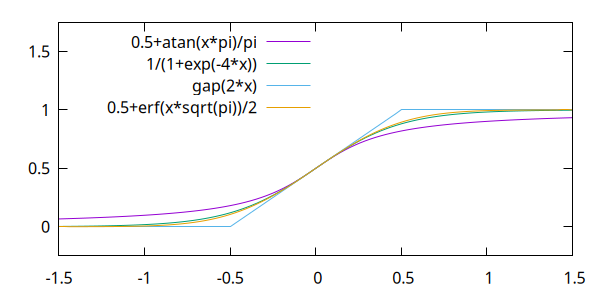
\includegraphics[width=0.5\linewidth]{f/plot_heavisides.png}
	\caption{Plots of the ``smooth heavisides''~$\sigma$ implemented in
	our program.  In all cases the parameter is set to~$1$, which
	corresponds to a slope of~$1$ at the origin.}
	\label{fig:heavisides}
\end{figure}



\section{Implementation}

Discrete implementation for a small support kernel, written in C

{\small
\begin{verbatim}
krt [options] KERNEL [IN [OUT]]

IN : input image (by default, stdin)
OUT : output image of the same size as the input (by default, stdout)
KERNEL : string that specifies the kernel k  Examples:

"file.npy" : the kernel is given by a numeric array, the center is at the
center of the image

"gauss:S" : the kernel is a gaussian of that sigma=S (in pixels)

"disk:R" : disk of radius R

"rectangle:N" : centered rectangle of size (2M+1)x(2M+1), where M=floor(N)

options:

-p 0 : getpixel = 0 outside the original image domain
-p 1 : getpixel = nearest neighbor
-p 2 : getpixel = symmetric extension
... (periodic, etc)

\end{verbatim}
}

Generic implementation as a 3d convolution (consider the problem of
gray-scale sampling!), written in C

{\small
\begin{verbatim}
krt3d [options] KERNEL [IN [OUT]]

IN : input image (by default, stdin)
OUT : output image of the same size as the input (by default, stdout)
KERNEL : string that specifies the kernel k  Examples:

"file.npy" : the kernel is given by a numeric array, the center is at the
center of the image, extended by zero outside of its domain

"gauss:S" : the kernel is a gaussian of that sigma=S (in pixels)

"riesz:S" : riesz kernel of parameter S

options:

-s 255 : gray-scale factor
-n 256 : number of gray-scale bins

future:
-h s : gray-level filtering parameter

\end{verbatim}
}

Verification that both implementations give the same result

Comparison of both implementations (table of running times depending on
kernel size/number of gray levels?)

\section{Examples and applications}

\subsection{Experiment: Adelson checkerboard }

% f/adelson.png
%SCRIPT ./krt square5  f/adelson.png |qauto -p 0 - f/adelson_sq5.png
%SCRIPT ./krt gauss5   f/adelson.png |qauto -p 0 - f/adelson_g5.png
%SCRIPT ./krt landc25  f/adelson.png |qauto -p 0 - f/adelson_l25.png
%SCRIPT ./krt square5 -h gap2 f/adelson.png|qauto -p 0 - f/adelson_sq5_gap2.png
%SCRIPT ./krt gauss5  -h gap2 f/adelson.png|qauto -p 0 - f/adelson_g5_gap2.png
%SCRIPT ./krt landc25 -h gap2 f/adelson.png|qauto -p 0 - f/adelson_l25_gap2.png
%SCRIPT ./krt square5 -h gap10 f/adelson.png|qauto -p 0 - f/adelson_sq5_gap10.png
%SCRIPT ./krt gauss5  -h gap10 f/adelson.png|qauto -p 0 - f/adelson_g5_gap10.png
%SCRIPT ./krt landc25 -h gap10 f/adelson.png|qauto -p 0 - f/adelson_l25_gap10.png
%SCRIPT ./krt square5 -h gap20 f/adelson.png|qauto -p 0 - f/adelson_sq5_gap20.png
%SCRIPT ./krt gauss5  -h gap20 f/adelson.png|qauto -p 0 - f/adelson_g5_gap20.png
%SCRIPT ./krt landc25 -h gap20 f/adelson.png|qauto -p 0 - f/adelson_l25_gap20.png
%SCRIPT ./krt square5 -h gap200 f/adelson.png|qauto -p 0 - f/adelson_sq5_gap200.png
%SCRIPT ./krt gauss5  -h gap200 f/adelson.png|qauto -p 0 - f/adelson_g5_gap200.png
%SCRIPT ./krt landc25 -h gap200 f/adelson.png|qauto -p 0 - f/adelson_l25_gap200.png

\begin{tabular}{cccc}
	& square 5 & gauss 5 & land25 \\
	h&
	\includegraphics[width=0.3\linewidth]{f/adelson_sq5.png} &
	\includegraphics[width=0.3\linewidth]{f/adelson_g5.png} &
	\includegraphics[width=0.3\linewidth]{f/adelson_l25.png} \\
	gap2&
	\includegraphics[width=0.3\linewidth]{f/adelson_sq5_gap2.png} &
	\includegraphics[width=0.3\linewidth]{f/adelson_g5_gap2.png} &
	\includegraphics[width=0.3\linewidth]{f/adelson_l25_gap2.png} \\
	gap10&
	\includegraphics[width=0.3\linewidth]{f/adelson_sq5_gap10.png} &
	\includegraphics[width=0.3\linewidth]{f/adelson_g5_gap10.png} &
	\includegraphics[width=0.3\linewidth]{f/adelson_l25_gap10.png} \\
	gap20&
	\includegraphics[width=0.3\linewidth]{f/adelson_sq5_gap20.png} &
	\includegraphics[width=0.3\linewidth]{f/adelson_g5_gap20.png} &
	\includegraphics[width=0.3\linewidth]{f/adelson_l25_gap20.png} \\
	gap200&
	\includegraphics[width=0.3\linewidth]{f/adelson_sq5_gap200.png} &
	\includegraphics[width=0.3\linewidth]{f/adelson_g5_gap200.png} &
	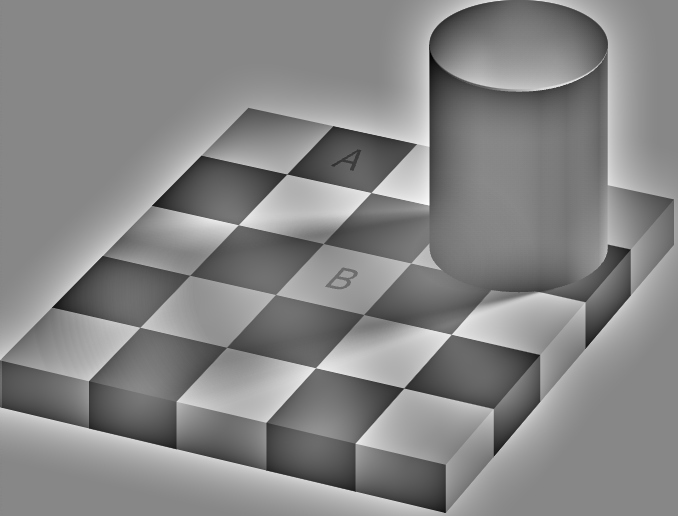
\includegraphics[width=0.3\linewidth]{f/adelson_l25_gap200.png} \\
\end{tabular}

%SCRIPT ./krt square3  f/adelson.png |qauto -p 0 - f/adelson_sq3.png
%SCRIPT ./krt square13  f/adelson.png |qauto -p 0 - f/adelson_sq13.png
%SCRIPT ./krt square33  f/adelson.png |qauto -p 0 - f/adelson_sq33.png
%SCRIPT ./krt gauss3   f/adelson.png |qauto -p 0 - f/adelson_g3.png
%SCRIPT ./krt gauss13   f/adelson.png |qauto -p 0 - f/adelson_g13.png
%SCRIPT ./krt gauss33   f/adelson.png |qauto -p 0 - f/adelson_g33.png
%SCRIPT ./krt landc3   f/adelson.png |qauto -p 0 - f/adelson_l3.png
%SCRIPT ./krt landc13   f/adelson.png |qauto -p 0 - f/adelson_l13.png
%SCRIPT ./krt landc33   f/adelson.png |qauto -p 0 - f/adelson_l33.png
\begin{tabular}{cccc}
	(heaviside)& square & gauss & land \\
	3&
	\includegraphics[width=0.3\linewidth]{f/adelson_sq3.png} &
	\includegraphics[width=0.3\linewidth]{f/adelson_g3.png} &
	\includegraphics[width=0.3\linewidth]{f/adelson_l3.png} \\
	13&
	\includegraphics[width=0.3\linewidth]{f/adelson_sq13.png} &
	\includegraphics[width=0.3\linewidth]{f/adelson_g13.png} &
	\includegraphics[width=0.3\linewidth]{f/adelson_l13.png} \\
	33&
	\includegraphics[width=0.3\linewidth]{f/adelson_sq33.png} &
	\includegraphics[width=0.3\linewidth]{f/adelson_g33.png} &
	\includegraphics[width=0.3\linewidth]{f/adelson_l33.png} \\
\end{tabular}

%SCRIPT ./krt square3  -h gap20 f/adelson.png |qauto -p 0 -  f/adelson_sq3_gap20.png
%SCRIPT ./krt square13 -h gap20  f/adelson.png |qauto -p 0 - f/adelson_sq13_gap20.png
%SCRIPT ./krt square33 -h gap20  f/adelson.png |qauto -p 0 - f/adelson_sq33_gap20.png
%SCRIPT ./krt gauss3   -h gap20 f/adelson.png |qauto -p 0 -  f/adelson_g3_gap20.png
%SCRIPT ./krt gauss13  -h gap20  f/adelson.png |qauto -p 0 - f/adelson_g13_gap20.png
%SCRIPT ./krt gauss33  -h gap20  f/adelson.png |qauto -p 0 - f/adelson_g33_gap20.png
%SCRIPT ./krt landc3   -h gap20 f/adelson.png |qauto -p 0 -  f/adelson_l3_gap20.png
%SCRIPT ./krt landc13  -h gap20  f/adelson.png |qauto -p 0 - f/adelson_l13_gap20.png
%SCRIPT ./krt landc33  -h gap20  f/adelson.png |qauto -p 0 - f/adelson_l33_gap20.png
\begin{tabular}{cccc}
	(gap20) & square & gauss  & land \\
	3&
	\includegraphics[width=0.3\linewidth]{f/adelson_sq3_gap20.png} &
	\includegraphics[width=0.3\linewidth]{f/adelson_g3_gap20.png} &
	\includegraphics[width=0.3\linewidth]{f/adelson_l3_gap20.png} \\
	13&
	\includegraphics[width=0.3\linewidth]{f/adelson_sq13_gap20.png} &
	\includegraphics[width=0.3\linewidth]{f/adelson_g13_gap20.png} &
	\includegraphics[width=0.3\linewidth]{f/adelson_l13_gap20.png} \\
	33&
	\includegraphics[width=0.3\linewidth]{f/adelson_sq33_gap20.png} &
	\includegraphics[width=0.3\linewidth]{f/adelson_g33_gap20.png} &
	\includegraphics[width=0.3\linewidth]{f/adelson_l33_gap20.png} \\
\end{tabular}

%SCRIPT ./krt square13 -h gap2 f/adelson.png |qeasy 0 1 - f/adelson_sq13_gap2.png
%SCRIPT ./krt square13 -h logistic2 f/adelson.png |qeasy 0 1 - f/adelson_sq13_logis2.png
%SCRIPT ./krt square13 -h arctan2 f/adelson.png |qeasy 0 1 - f/adelson_sq13_atan2.png
%SCRIPT ./krt square13 -h gap10 f/adelson.png |qeasy 0 1 - f/adelson_sq13_gap10.png
%SCRIPT ./krt square13 -h logistic10 f/adelson.png |qeasy 0 1 - f/adelson_sq13_logis10.png
%SCRIPT ./krt square13 -h arctan10 f/adelson.png |qeasy 0 1 - f/adelson_sq13_atan10.png
%SCRIPT ./krt square13 -h gap20 f/adelson.png |qeasy 0 1 - f/adelson_sq13_gap20.png
%SCRIPT ./krt square13 -h logistic20 f/adelson.png |qeasy 0 1 - f/adelson_sq13_logis20.png
%SCRIPT ./krt square13 -h arctan20 f/adelson.png |qeasy 0 1 - f/adelson_sq13_atan20.png
%SCRIPT ./krt square13 -h gap200 f/adelson.png |qeasy 0 1 - f/adelson_sq13_gap200.png
%SCRIPT ./krt square13 -h logistic200 f/adelson.png |qeasy 0 1 - f/adelson_sq13_logis200.png
%SCRIPT ./krt square13 -h arctan200 f/adelson.png |qeasy 0 1 - f/adelson_sq13_atan200.png
\begin{tabular}{cccc}
	(square 13) & gap & logistic & arctan \\
	gap2&
	\includegraphics[width=0.3\linewidth]{f/adelson_sq13_gap2.png} &
	\includegraphics[width=0.3\linewidth]{f/adelson_sq13_logis2.png} &
	\includegraphics[width=0.3\linewidth]{f/adelson_sq13_atan2.png} \\
	gap10&
	\includegraphics[width=0.3\linewidth]{f/adelson_sq13_gap10.png} &
	\includegraphics[width=0.3\linewidth]{f/adelson_sq13_logis10.png} &
	\includegraphics[width=0.3\linewidth]{f/adelson_sq13_atan10.png} \\
	gap20&
	\includegraphics[width=0.3\linewidth]{f/adelson_sq13_gap20.png} &
	\includegraphics[width=0.3\linewidth]{f/adelson_sq13_logis20.png} &
	\includegraphics[width=0.3\linewidth]{f/adelson_sq13_atan20.png} \\
	gap200&
	\includegraphics[width=0.3\linewidth]{f/adelson_sq13_gap200.png} &
	\includegraphics[width=0.3\linewidth]{f/adelson_sq13_logis200.png} &
	\includegraphics[width=0.3\linewidth]{f/adelson_sq13_atan200.png} \\
\end{tabular}



\subsection{Experiment: mach bands}

%SCRIPT plambda zero:500x120 ":i 50 / floor" -o f/mach.npy
%%SCRIPT plambda zero:500x120 ":i 50 / floor randg 0.01 * +" -o f/mach.npy
%%SCRIPT plambda zero:500x120 ":i 50 / floor randg 0.1 * +" -o f/mach.npy
%SCRIPT plambda f/mach.npy '7 - 14 * 127 +' -o f/mach.png

%SCRIPT export X="set term pngcairo size 500,200;unset key;unset xtics"
%SCRIPT cat f/mach.npy|(echo "$X";cline 0)|gnuplot >f/p_mach.png

%SCRIPT ./krt square21 f/mach.npy|qeasy 0 1 - f/mach_sq21.png
%SCRIPT ./krt square21 f/mach.npy|(echo "$X";cline 0)|gnuplot >f/p_mach_sq21.png

%SCRIPT ./krt gauss7 f/mach.npy|qeasy 0 1 - f/mach_g7.png
%SCRIPT ./krt gauss7 f/mach.npy|(echo "$X";cline 0)|gnuplot >f/p_mach_g7.png

%SCRIPT ./krt cauchy3 f/mach.npy|qeasy 0 1 - f/mach_c3.png
%SCRIPT ./krt cauchy3 f/mach.npy|(echo "$X";cline 0)|gnuplot >f/p_mach_c3.png

%SCRIPT ./krt landc40 f/mach.npy|qeasy 0 1 - f/mach_la.png
%SCRIPT ./krt landc40 f/mach.npy|(echo "$X";cline 0)|gnuplot >f/p_mach_la.png


%SCRIPT plambda f/mach.npy ":i 0.004 * +" -o f/umach.npy
%SCRIPT plambda f/umach.npy '7 - 14 * 127 +' -o f/umach.png
%SCRIPT cat f/umach.npy|(echo "$X";cline 0)|gnuplot >f/p_umach.png
%SCRIPT ./krt square21 f/umach.npy|qeasy 0 1 - f/umach_sq21.png
%SCRIPT ./krt square21 f/umach.npy|(echo "$X";cline 0)|gnuplot >f/p_umach_sq21.png
%SCRIPT ./krt gauss7 f/umach.npy|qeasy 0 1 - f/umach_g7.png
%SCRIPT ./krt gauss7 f/umach.npy|(echo "$X";cline 0)|gnuplot >f/p_umach_g7.png
%SCRIPT ./krt cauchy3 f/umach.npy|qeasy 0 1 - f/umach_c3.png
%SCRIPT ./krt cauchy3 f/umach.npy|(echo "$X";cline 0)|gnuplot >f/p_umach_c3.png
%SCRIPT ./krt landc40 f/umach.npy|qeasy 0 1 - f/umach_la.png
%SCRIPT ./krt landc40 f/umach.npy|(echo "$X";cline 0)|gnuplot >f/p_umach_la.png

%SCRIPT plambda f/mach.npy ":i 0.004 * -" -o f/dmach.npy
%SCRIPT plambda f/dmach.npy '7 - 14 * 127 +' -o f/dmach.png
%SCRIPT cat f/dmach.npy|(echo "$X";cline 0)|gnuplot >f/p_dmach.png
%SCRIPT ./krt square21 f/dmach.npy|qeasy 0 1 - f/dmach_sq21.png
%SCRIPT ./krt square21 f/dmach.npy|(echo "$X";cline 0)|gnuplot >f/p_dmach_sq21.png
%SCRIPT ./krt gauss7 f/dmach.npy|qeasy 0 1 - f/dmach_g7.png
%SCRIPT ./krt gauss7 f/dmach.npy|(echo "$X";cline 0)|gnuplot >f/p_dmach_g7.png
%SCRIPT ./krt cauchy3 f/dmach.npy|qeasy 0 1 - f/dmach_c3.png
%SCRIPT ./krt cauchy3 f/dmach.npy|(echo "$X";cline 0)|gnuplot >f/p_dmach_c3.png
%SCRIPT ./krt landc40 f/dmach.npy|qeasy 0 1 - f/dmach_la.png
%SCRIPT ./krt landc40 f/dmach.npy|(echo "$X";cline 0)|gnuplot >f/p_dmach_la.png

\begin{figure}
	\begin{tabular}{cc}
		\includegraphics[width=0.45\linewidth]{f/mach.png} &
		\includegraphics[width=0.45\linewidth]{f/p_mach.png} \\
		\includegraphics[width=0.45\linewidth]{f/mach_sq21.png} &
		\includegraphics[width=0.45\linewidth]{f/p_mach_sq21.png} \\
		\includegraphics[width=0.45\linewidth]{f/mach_g7.png} &
		\includegraphics[width=0.45\linewidth]{f/p_mach_g7.png} \\
		\includegraphics[width=0.45\linewidth]{f/mach_c3.png} &
		\includegraphics[width=0.45\linewidth]{f/p_mach_c3.png} \\
		\includegraphics[width=0.45\linewidth]{f/mach_la.png} &
		\includegraphics[width=0.45\linewidth]{f/p_mach_la.png} \\
	\end{tabular}
	\caption{\label{fig:machnonoise}
		Mach bands without noise, various kernels.
	}
\end{figure}

\begin{figure}
	\begin{tabular}{cc}
		\includegraphics[width=0.45\linewidth]{f/umach.png} &
		\includegraphics[width=0.45\linewidth]{f/p_umach.png} \\
		\includegraphics[width=0.45\linewidth]{f/umach_sq21.png} &
		\includegraphics[width=0.45\linewidth]{f/p_umach_sq21.png} \\
		\includegraphics[width=0.45\linewidth]{f/umach_g7.png} &
		\includegraphics[width=0.45\linewidth]{f/p_umach_g7.png} \\
		\includegraphics[width=0.45\linewidth]{f/umach_c3.png} &
		\includegraphics[width=0.45\linewidth]{f/p_umach_c3.png} \\
		\includegraphics[width=0.45\linewidth]{f/umach_la.png} &
		\includegraphics[width=0.45\linewidth]{f/p_umach_la.png} \\
	\end{tabular}
	\caption{\label{fig:machup}
		Mach bands with up-ramp, various kernels.
	}
\end{figure}

\begin{figure}
	\begin{tabular}{cc}
		\includegraphics[width=0.45\linewidth]{f/dmach.png} &
		\includegraphics[width=0.45\linewidth]{f/p_dmach.png} \\
		\includegraphics[width=0.45\linewidth]{f/dmach_sq21.png} &
		\includegraphics[width=0.45\linewidth]{f/p_dmach_sq21.png} \\
		\includegraphics[width=0.45\linewidth]{f/dmach_g7.png} &
		\includegraphics[width=0.45\linewidth]{f/p_dmach_g7.png} \\
		\includegraphics[width=0.45\linewidth]{f/dmach_c3.png} &
		\includegraphics[width=0.45\linewidth]{f/p_dmach_c3.png} \\
		\includegraphics[width=0.45\linewidth]{f/dmach_la.png} &
		\includegraphics[width=0.45\linewidth]{f/p_dmach_la.png} \\
	\end{tabular}
	\caption{\label{fig:machdown}
		Mach bands with down-ramp, various kernels.
	}
\end{figure}

TODO (points A3' and A3'' in the TODO list): add the experiments above (mach
bands), with a smooth step function.  This renders the method non-contrast
invariant, but continuous.  And maybe closer to our perception (the three
cases of mach bands look identical before and after the krt).

\subsection{Experiment: Effect of the scale parameter}

show square rank scale-space (using square of varying side)

show gaussian rank scale-space


\subsection{Experiment: Comparison of different kernels}

maybe show other kernel scalespaces ?

multi-scale kernels (e.g. riesz scale space)

non-isotropic kernels ?
(ref. hirschmuller "7x5")



\subsection{Experiment: further parameter exploration}

Pick a reference image:
perlin noise of grain s + gaussian blur of intensity r
filter this image with gaussian-gaussian krt, varying botht parameters,
observe the effects depending on whether the parameters are larger/smaller
than s/r.


\subsection{Application: local image normalization}

sub-application: adaptive thresholding
\url{https://docs.opencv.org/4.x/d7/d4d/tutorial_py_thresholding.html}

\subsection{Application: noise uniformization}

After applying the KRT, noise becomes uniform.

This is an important difference between the original discrete rank transform
and the kernel rank transform (with a non-constant kernel like the
gaussian).  Both transforms produce an image with a locally uniform
histogram, as much as they can.  But the original rank transform, by
construction, produces an image whose values are integers between 1
and~$N^2$, while the smooth kernel rank transform will give generally
different floating point numbers.  Even for kernels with small support, it
produces images whose histogram is uniform, but much more finely quantized.

%SCRIPT plambda zero:256x256 "randg" -o f/randg.npy
%SCRIPT ./krt square7 f/randg.npy |plambda "48 * 1 + round"| ghisto -p | gnuplot > f/randg_k7_h.png
%SCRIPT ./krt gauss1.5 f/randg.npy |plambda '1000 * round 1000 /'| ghisto -p | gnuplot > f/randg_g15_h.png
\begin{figure}[p]
	\begin{tabular}{cc}
		\includegraphics[width=0.49\linewidth]{f/randg_k7_h.png} &
		\includegraphics[width=0.49\linewidth]{f/randg_g15_h.png} \\
		rank transform~$7x7$ &
		KRT~$\sigma=1.5$
	\end{tabular}
	\caption{\label{fig:histograms}
	Histograms of white Gaussian noise uniformized with a classical
	rank transform of size~$7x7$ and a kernel rank transform with a
	Gaussian of~$\sigma=1.5$ (with the same $7\times7$ support).
	}
\end{figure}


\subsection{Application: image comparison}

If we have images of the same scene with very different dynamic ranges, the
rank transform allows to compare them directly.   


\section{References}

\bibliographystyle{plain}
\bibliography{refs}


\end{document}


% vim:set tw=76 filetype=tex spell spelllang=en:
